\documentclass[10pt]{beamer}

\usetheme[titleformat=smallcaps]{metropolis}
\usepackage{appendixnumberbeamer}

\usepackage{booktabs}
\usepackage[scale=2]{ccicons}
\usepackage{tcolorbox}

%\usepackage{minted}
%\usemintedstyle{trac}

\usepackage{pgfplots}
\usepgfplotslibrary{dateplot}

\usepackage{xspace}
\newcommand{\themename}{\textbf{\textsc{metropolis}}\xspace}


\usepackage{subfig}
\usepackage[absolute,overlay]{textpos}
\usepackage{tikz}



\usepackage{times}
\usepackage{amsmath}
\usepackage{verbatim}
\usetikzlibrary{arrows,shapes}


\usepackage{mathtools}

\newcommand{\verteq}{\rotatebox{90}{$\,=$}}
\newcommand{\equalto}[2]{\underset{\scriptstyle\overset{\mkern4mu\huge \verteq}{#2}}{#1}}


\newcommand{\bra}[1]{\left\langle #1\right|}
\newcommand{\ket}[1]{\left| #1\right\rangle}
\newcommand{\braket}[2]{\langle #1 \mid #2 \rangle}
\newcommand{\avg}[1]{\left< #1 \right>}

\newcommand{\ii}{\mathrm{i}}



%%%%%%%%%%%%%%%%%%%%%%%%%
%%%%% For Timeline %%%%%%

% http://tex.stackexchange.com/questions/196794/how-can-you-create-a-vertical-timeline

%\usepackage[T1]{fontenc}
\usepackage[utf8]{inputenc}
\usepackage{charter}
\usepackage{environ}
\usepackage{tikz}
\usetikzlibrary{calc,matrix}

\makeatletter
\let\matamp=&
\catcode`\&=13
\makeatletter
\def&{\iftikz@is@matrix
  \pgfmatrixnextcell
  \else
  \matamp
  \fi}
\makeatother

\newcounter{lines}
\def\endlr{\stepcounter{lines}\\}

\newcounter{vtml}
\setcounter{vtml}{0}

\newif\ifvtimelinetitle
\newif\ifvtimebottomline
\tikzset{description/.style={
  column 2/.append style={#1}
 },
 timeline color/.store in=\vtmlcolor,
 timeline color=red!80!black,
 timeline color st/.style={fill=\vtmlcolor,draw=\vtmlcolor},
 use timeline header/.is if=vtimelinetitle,
 use timeline header=false,
 add bottom line/.is if=vtimebottomline,
 add bottom line=false,
 timeline title/.store in=\vtimelinetitle,
 timeline title={},
 line offset/.store in=\lineoffset,
 line offset=4pt,
}

\NewEnviron{vtimeline}[1][]{%
\setcounter{lines}{1}%
\stepcounter{vtml}%
\begin{tikzpicture}[column 1/.style={anchor=east},
 column 2/.style={anchor=west},
 text depth=0pt,text height=1ex,
 row sep=1ex,
 column sep=1em,
 #1
]
\matrix(vtimeline\thevtml)[matrix of nodes]{\BODY};
\pgfmathtruncatemacro\endmtx{\thelines-1}
\path[timeline color st] 
($(vtimeline\thevtml-1-1.north east)!0.5!(vtimeline\thevtml-1-2.north west)$)--
($(vtimeline\thevtml-\endmtx-1.south east)!0.5!(vtimeline\thevtml-\endmtx-2.south west)$);
\foreach \x in {1,...,\endmtx}{
 \node[circle,timeline color st, inner sep=0.15pt, draw=white, thick] 
 (vtimeline\thevtml-c-\x) at 
 ($(vtimeline\thevtml-\x-1.east)!0.5!(vtimeline\thevtml-\x-2.west)$){};
 \draw[timeline color st](vtimeline\thevtml-c-\x.west)--++(-3pt,0);
 }
 \ifvtimelinetitle%
  \draw[timeline color st]([yshift=\lineoffset]vtimeline\thevtml.north west)--
  ([yshift=\lineoffset]vtimeline\thevtml.north east);
  \node[anchor=west,yshift=16pt,font=\large]
   at (vtimeline\thevtml-1-1.north west) 
   {\textsc{Timeline \thevtml}: \textit{\vtimelinetitle}};
 \else%
  \relax%
 \fi%
 \ifvtimebottomline%
   \draw[timeline color st]([yshift=-\lineoffset]vtimeline\thevtml.south west)--
  ([yshift=-\lineoffset]vtimeline\thevtml.south east);
 \else%
   \relax%
 \fi%
\end{tikzpicture}
}


%%%% Timeline END %%%%%%%
%%%%%%%%%%%%%%%%%%%%%%%%%


\title{Neutrino Oscillations in Matter}
\subtitle{PhD Candidacy Exam}
\date{\today}
\author{Lei Ma\\
{\bf{Supervisor}}: Huaiyu Duan}
\institute{Department of Physics\\
UNM}
% \titlegraphic{\hfill
\includegraphics[height=1.5cm]{logo.pdf}}

\begin{document}

\maketitle

\begin{frame}{Table of Contents}
  \setbeamertemplate{section in toc}[sections numbered]
  \tableofcontents
\end{frame}

\section{Introduction}


\subsection{History of Neutrinos}

\begin{frame}[fragile]{Neutrino Timeline}


\begin{vtimeline}[description={text width=\textwidth}, 
 row sep=2ex, 
 use timeline header,
 timeline title={(Partial) History of Neutrino}]
1930 & Pauli, letter to "Radioactive Ladies and Gentlemen"\endlr
1933 & Fermi, the name "neutrino" \endlr
1956 & Reines \& Cowan, first neutrino evidence \endlr
1957 & \textbf{Pontecorvo, theory of neutrino oscillations} \endlr
1968 & Homestake, first solar neutrino detection \endlr
1969 & Gribov \& Pontecorvo, solar neutrino oscillations \endlr
1978 \& 1985 & \textbf{Wolfenstein \& Mikheyev \& Smirnov, MSW effect} \endlr
1987 & Kamioka mine \& Morton salt mine, SN1987A neutrino\endlr
1998 \& 2001 & Super-Kamiokande \& SNO, solar neutrino oscillations \endlr
\end{vtimeline}


\end{frame}







%%%% Neutrino as a Particle
\subsection{What is neutrino?}

\begin{frame}{What is neutrino?}

\begin{figure}
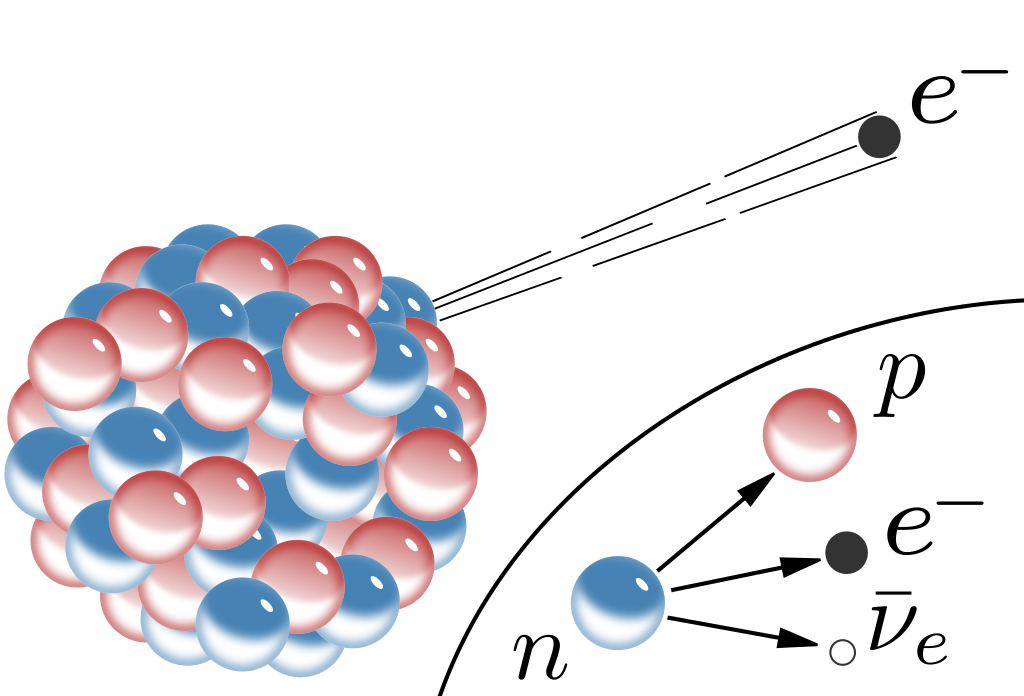
\includegraphics[width=0.9\linewidth,height=0.9\textheight,keepaspectratio]{assets/beta-decay.png}
\caption{Beta decay and antineutrino production. Source: Beta\_Decay@Wikipedia}
\end{figure}


\end{frame}




\begin{frame}{What is neutrino?}

\begin{minipage}[\textheight]{\textwidth}
\begin{columns}[T]

\begin{column}{0.6\textwidth}
\begin{figure}
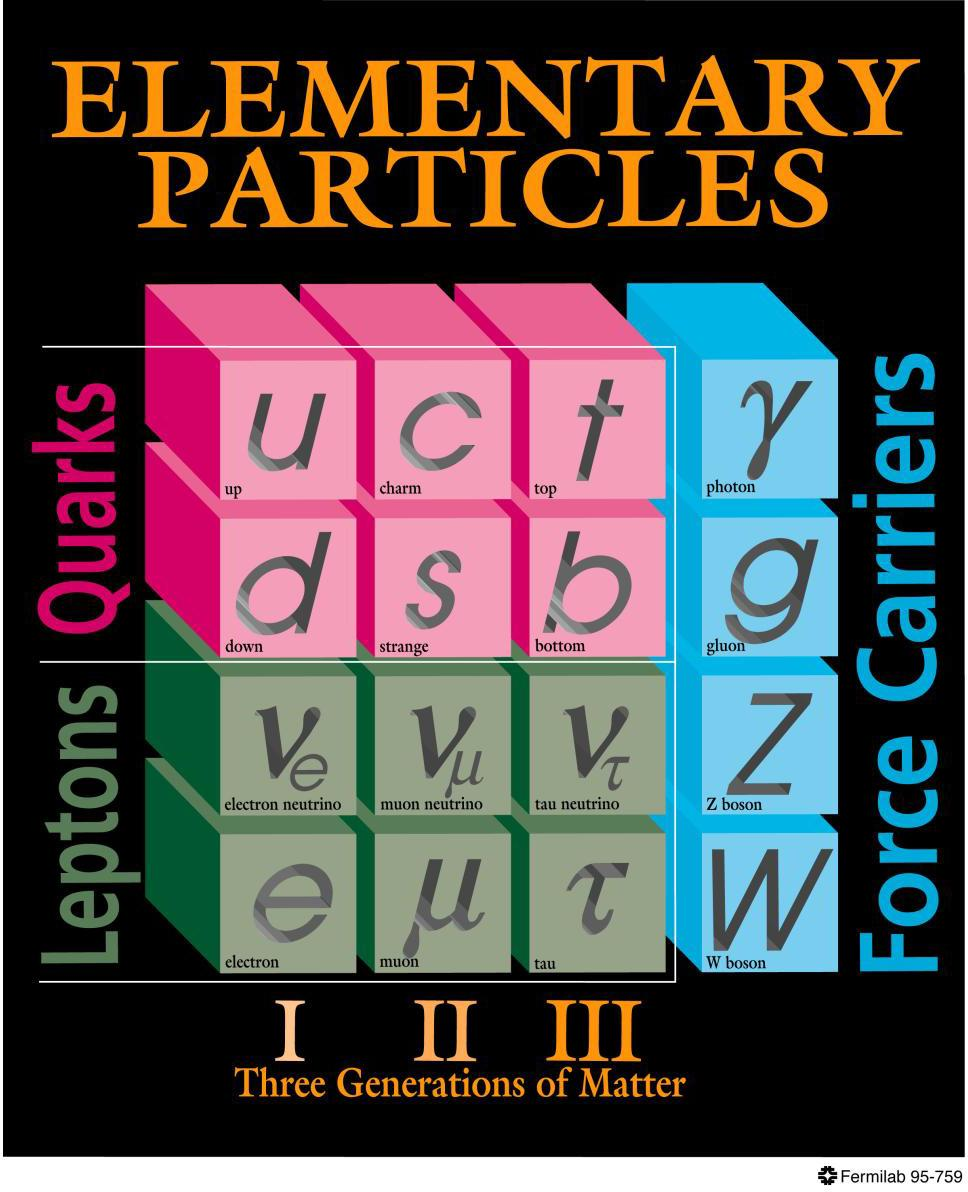
\includegraphics[width=0.9\linewidth,height=0.8\textheight,keepaspectratio]{assets/elementary-particles.jpg}
\caption{Table of elementary particles. Source: Fermilab} % http://www-d0.fnal.gov/Run2Physics/WWW/results/final/TOP/T06C/T06C.html
\end{figure}
\end{column}

\begin{column}{0.4\textwidth}


    \begin{itemize}
    \item[] Neutrinos are
    \item Fermions,
    \item electrically neutral,
    \item \textbf{light}.
    \end{itemize}



\only<1-1>{
\begin{figure}
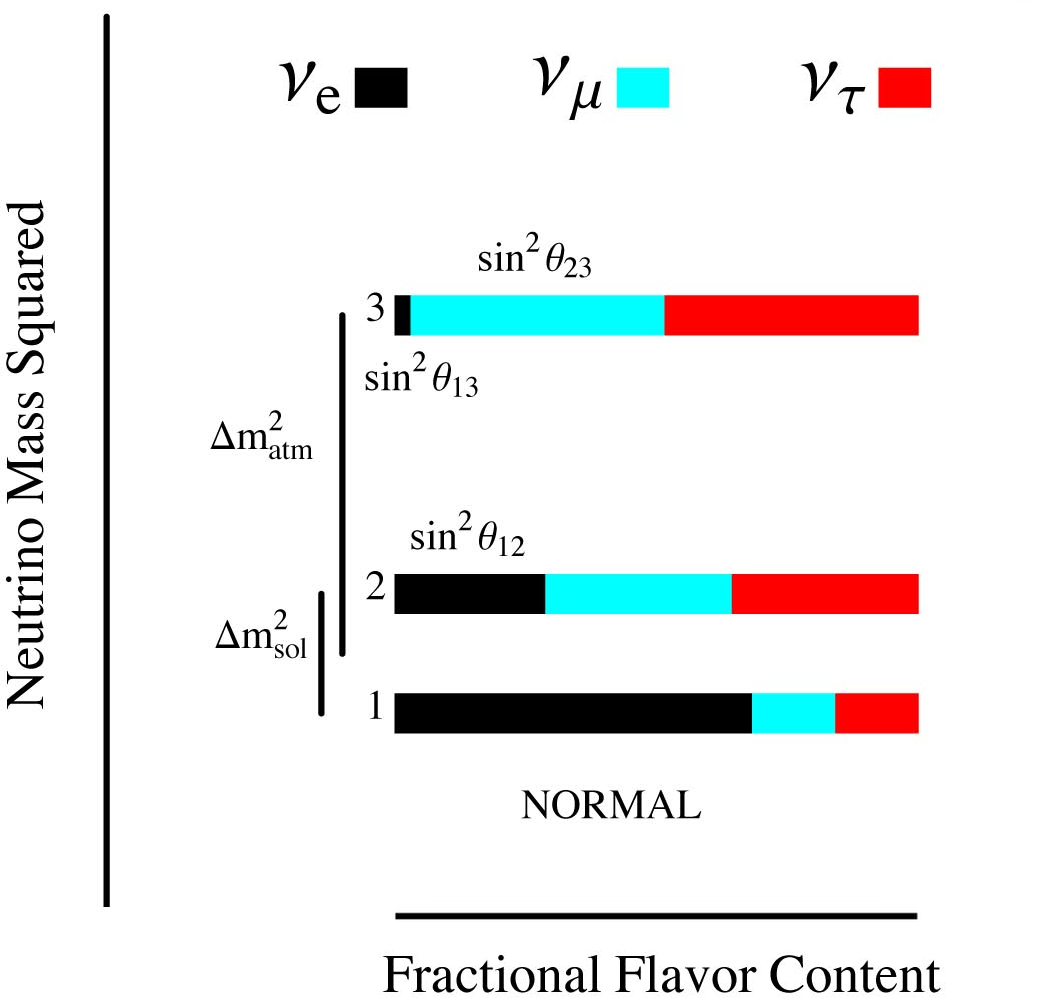
\includegraphics[width=\textwidth]{assets/neutrino-normal-hierarchy.png}
\caption*{Olga Mena \& Stephen Parke, 2004}
\end{figure}
}

\only<2-2>{
\begin{figure}
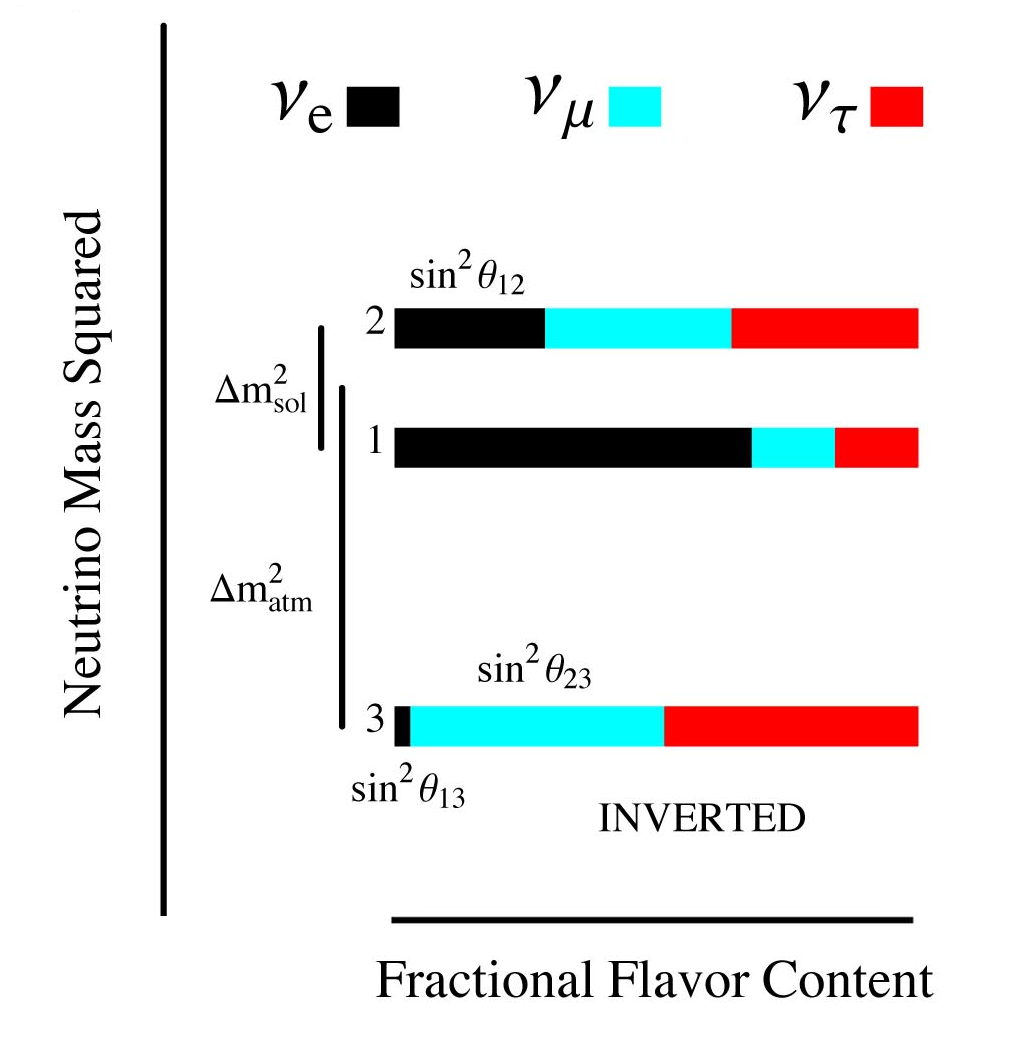
\includegraphics[width=\textwidth]{assets/neutrino-inverted-hierarchy.png}
\caption*{Olga Mena \& Stephen Parke, 2004}
\end{figure}
}

\end{column}


\end{columns}
\end{minipage}

\end{frame}



%%%%% Neutrino Oscillations %%%%%%%%%

\subsection{Neutrino oscillation}


\begin{frame}{What is neutrino oscillation?}


\begin{figure}
  \centering
{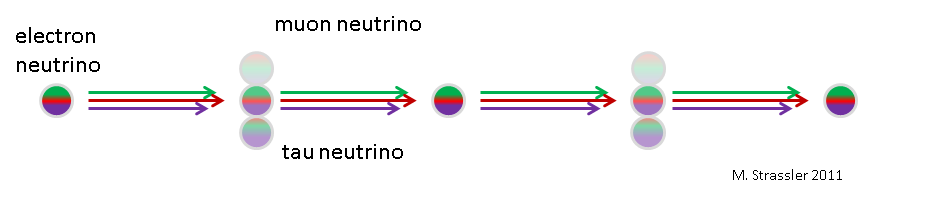
\includegraphics[width=\linewidth,height=0.22\textheight,keepaspectratio]{assets/neutrino-oscillations-illustration.png} }
%http://profmattstrassler.com/articles-and-posts/particle-physics-basics/neutrinos/neutrino-types-and-neutrino-oscillations/
\vfill
\pause
{
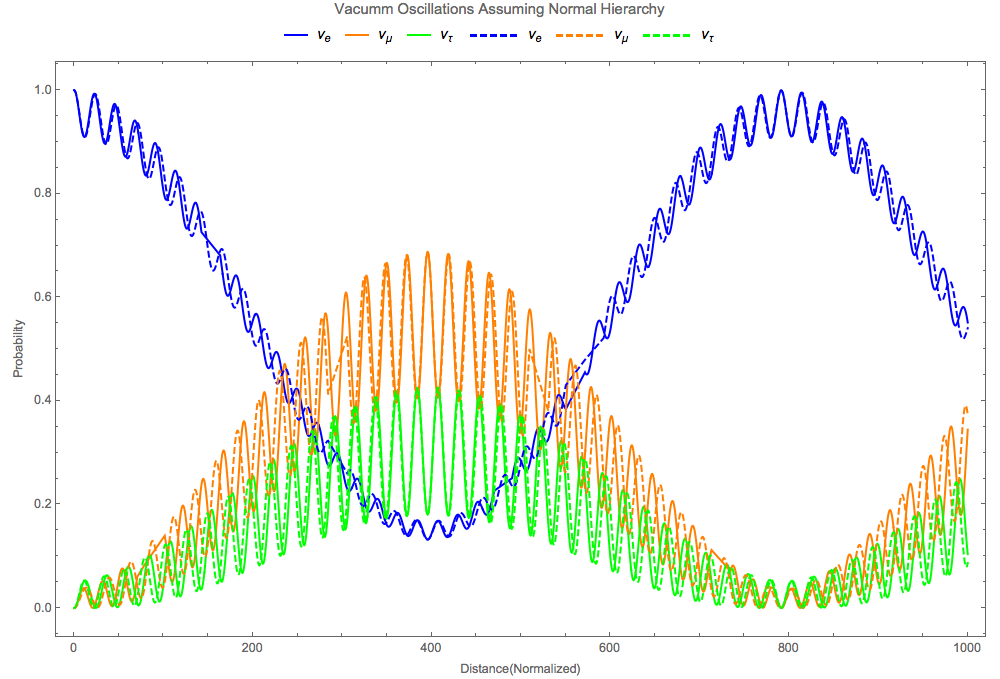
\includegraphics[width=0.7\linewidth,height=0.9\textheight,keepaspectratio]{assets/vacuum-oscillations-survival-probability.png}
}
\caption{Neutrino oscillation. Source: Neutrino\_oscillation@Wikipedia \textbf{SHOULD CHANGE TO A CUSTOMIZED FIGURE} }

\end{figure}



\end{frame}



\begin{frame}{What is neutrino oscillation?}


\setcounter{figure}{\thefigure-1}  
\begin{figure}
  \centering
{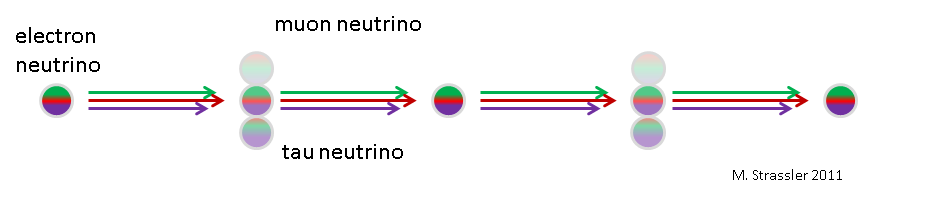
\includegraphics[width=\linewidth,height=0.22\textheight,keepaspectratio]{assets/neutrino-oscillations-illustration.png} }
%http://profmattstrassler.com/articles-and-posts/particle-physics-basics/neutrinos/neutrino-types-and-neutrino-oscillations/
\vfill
{
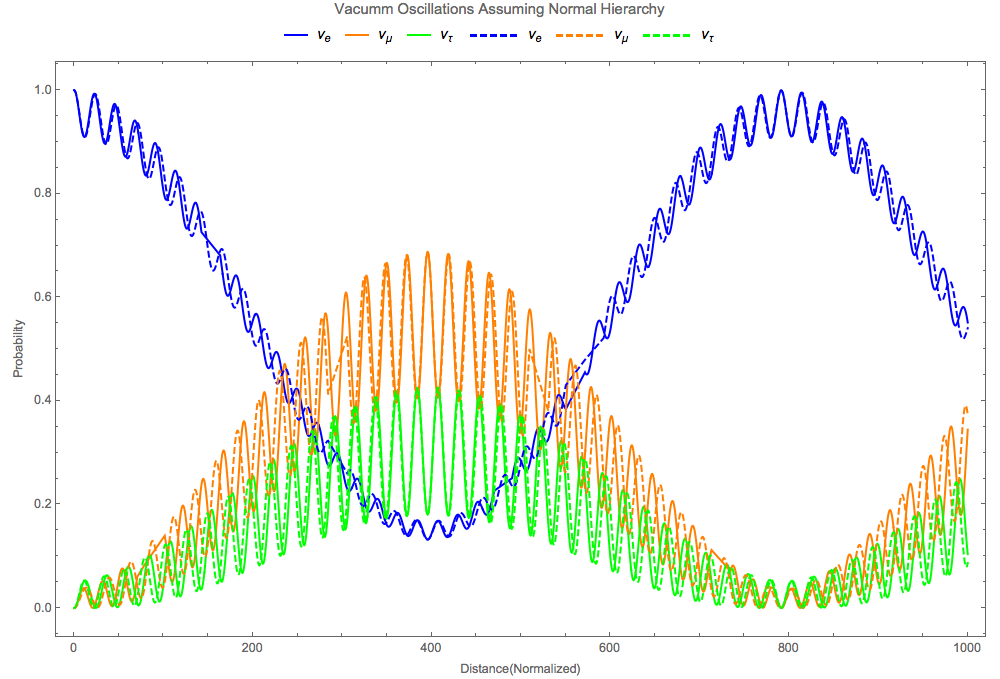
\includegraphics[width=0.7\linewidth,height=0.9\textheight,keepaspectratio]{assets/vacuum-oscillations-survival-probability.png}
}
\caption{Neutrino oscillation. Source: Neutrino\_oscillation@Wikipedia \textbf{SHOULD CHANGE TO A CUSTOMIZED FIGURE} }

\end{figure}


\begin{textblock*}{64mm}(32mm,0.4\textheight)

\metroset{block=fill}
\begin{tcolorbox}
\centering
\begin{equation*}
  \equalto{\textbf{\large Neutrino Oscillations} }{ \textbf{\large Neutrino Flavor Conversion } }
\end{equation*}

\vspace{1em}
\end{tcolorbox}
\end{textblock*}


\end{frame}




%%%%%% Why Neutrinos Oscillate? %%%%%%%%%


% For every picture that defines or uses external nodes, you'll have to
% apply the 'remember picture' style. To avoid some typing, we'll apply
% the style to all pictures.
\tikzstyle{every picture}+=[remember picture]

% By default all math in TikZ nodes are set in inline mode. Change this to
% displaystyle so that we don't get small fractions.
\everymath{\displaystyle}


\begin{frame}[fragile]{Why Do Neutrinos Oscillate?}

\begin{tcolorbox}[title=Equation of Motion]

\begin{equation*}
i\partial_x \Psi = \mathbf H \Psi
\end{equation*}

\end{tcolorbox}




\begin{itemize}
\item Choose a proper basis: Hamiltonian diagonalized basis/mass eigenbasis/propagation eigenbasis.

\item
\begin{equation*}
    \mathbf H = - \frac{\omega_v}{2}\boldsymbol{\sigma_3}, \qquad \text{where } \omega_v = \frac{\delta m^2}{2E}.
\end{equation*}



\item The system can be solved given initial condition of the wave function $(\psi_1(0),\psi_2(0))^T$,
\begin{equation*}
    \begin{pmatrix}
    \psi_1(t) \\
    \psi_2(t)
    \end{pmatrix} = \begin{pmatrix}
    \psi_1(0) \exp\left( \ii  \omega_v x /2 \right) \\
    \psi_2(0) \exp\left( -\ii  \omega_v x/2 \right)
    \end{pmatrix} 
\end{equation*}


\end{itemize}




\end{frame}


%%%%%%%%%



\begin{frame}[fragile]{Why Do Neutrinos Oscillate?}
\setbeamercovered{transparent}

\begin{tcolorbox}[title=Flavor basis]


Neutrino state in flavor basis $(\psi_e, \psi_x)^T$ is related to state in energy eigenbasis $(\psi_1,\psi_2)^T$ through
\begin{equation*}
\begin{pmatrix}\nu_e \\ \nu_x\end{pmatrix} = \begin{pmatrix}  \cos\theta  & \sin\theta \\ -\sin\theta  & \cos\theta \end{pmatrix}   \begin{pmatrix}\nu_1 \\ \nu_2\end{pmatrix}
\end{equation*}

\end{tcolorbox}

\pause

\begin{tcolorbox}[title=Hamiltonian $\mathbf H$]

\begin{columns}[T] % align columns
\begin{column}{.49\textwidth}
\color{teal}\rule{\linewidth}{4pt}
\centering Mass eigenstate basis


\begin{align*}
&\frac{\omega_v}{2}\begin{pmatrix}
-1  & 0 \\
0 & 1
\end{pmatrix}\\
=&
-\frac{\omega_v}{2}\boldsymbol{ \sigma_3 }
\end{align*}



\end{column}%
\hfill%

\begin{column}{.49\textwidth}
\color{olive}\rule{\linewidth}{4pt}
\centering Flavor eigenstate basis

\begin{align*}
&\frac{\omega_v}{2}\begin{pmatrix} -\cos 2\theta_v & \sin 2 \theta_v \\ \sin 2\theta_v & \cos 2\theta_v  \end{pmatrix} \\
=&
\frac{\omega_v}{2}\left( - \cos 2\theta_v\boldsymbol{ \sigma_3 } + \sin 2\theta_v \boldsymbol{\sigma_1} \right)
\end{align*}

\end{column}%
\end{columns}

\end{tcolorbox}



\end{frame}





\begin{frame}[fragile]
  \frametitle{Nature of Neutrino Oscillation}
\setbeamercovered{transparent}

\onslide<1->{
\begin{tcolorbox}[title=What is the cause of oscillation?]
As long as flavor eigenstates are NOT energy eigenstates, neutrino oscillations can happen.
\end{tcolorbox}
}

\onslide<1->{
\begin{tcolorbox}[title=Basis]
\begin{description}
\item[Energy Eigenbasis] Diagonalized Hamiltonian
\item[Flavor Eigenbasis] Eigenstates of weak interaction
\end{description}
\end{tcolorbox}
}


%%% Pause here
%\pasue

\onslide<2->{
\begin{tcolorbox}[title=Mixing Angle and Eigenenergies]
\alert{Change mixing angles $\to$ change mixing amplitude\\
Change energy eigenstates $\to$ mixing frequency}

\begin{equation*}
P(\ket{\nu_e}\to\ket{\nu_x})  = \frac{1}{2} \sin^2(2\theta_v) \left[ 1- \cos \left( \omega_v x \right) \right]
\end{equation*}
\end{tcolorbox}
}

\end{frame}




%%%%%%%%%%%%%%%%%%%%%%%%%%%%%%%%%%%%%%%%%%%%%%%%%%%%%%%%%%%%%%%%%%
%%%%%%%%%%%%%%%%%%%% Matter Effect %%%%%%%%%%%%%%%


\section{Matter Effect}


\subsection{Matter Interaction}


\begin{frame}{Matter Interaction}


\begin{tcolorbox}[title=PLACEHOLDER]
SHOULD ADD IN WHY MATTER INTERACTION IS LIKE THIS test math $\frac{A}{B}$
\end{tcolorbox}


\end{frame}





% For every picture that defines or uses external nodes, you'll have to
% apply the 'remember picture' style. To avoid some typing, we'll apply
% the style to all pictures.
\tikzstyle{every picture}+=[remember picture]


% By default all math in TikZ nodes are set in inline mode. Change this to
% displaystyle so that we don't get small fractions.
\everymath{\displaystyle}



\begin{frame}{Matter Interaction}
\tikzstyle{na} = [baseline=-.5ex]




\begin{itemize}
    \item[] Hamiltonian with Matter Interaction in Flavor Basis:
        \tikz[na] \node[coordinate] (n1) {};
\end{itemize}


\only<1-1>{
\begin{equation*}
    \mathbf{H} = 
    \tikz[baseline]{
            \node[fill=blue!20,anchor=base] (t1)
            {$ \frac{\omega_v}{2}\begin{pmatrix} -\cos 2\theta_v & \sin 2 \theta_v \\ \sin 2\theta_v & \cos 2\theta_v  \end{pmatrix} $}
            } + 
            \tikz[baseline]{
            \node[fill=red!20, anchor=base] (t2)
            {$ 
            \sqrt{2}G_F n_e(x) \begin{pmatrix}
            1 & 0 \\
            0 & 0
            \end{pmatrix}
            $};
        }
\end{equation*}



}




\only<2-2>{
\begin{equation*}
    \mathbf{H} = 
    \tikz[baseline]{
            \node[fill=blue!20,anchor=base] (t1)
            {$ \frac{\omega_v}{2}\begin{pmatrix} -\cos 2\theta_v & \sin 2 \theta_v \\ \sin 2\theta_v & \cos 2\theta_v  \end{pmatrix} $}
            } + 
            \tikz[baseline]{
            \node[fill=red!20, anchor=base] (t2)
            {$ 
            \frac{\sqrt{2}G_F n_e(x)}{2} \begin{pmatrix}
            1 & 0 \\
            0 & -1
            \end{pmatrix}
            $};
        }
\end{equation*}

}

\only<3-3>{
\begin{equation*}
    \mathbf{H} = 
    \tikz[baseline]{
            \node[fill=blue!20,anchor=base] (t1)
            {$ \frac{\omega_v}{2}\left( - \cos 2\theta_v \boldsymbol{\sigma_3} + \sin 2\theta_v \boldsymbol{\sigma_1} \right) $}
            } + 
            \tikz[baseline]{
            \node[fill=red!20, anchor=base] (t2)
            {$ 
            \frac{\sqrt{2}G_F n_e(x)}{2} \boldsymbol{\sigma_3}
            $};
        }
\end{equation*}

}

\only<4->{
\begin{equation*}
    \mathbf{H} = 
    \tikz[baseline]{
            \node[fill=blue!20,anchor=base] (t1)
            {$ \frac{\omega_v}{2}\left( - \cos 2\theta_v \boldsymbol{\sigma_3} + \sin 2\theta_v \boldsymbol{\sigma_1} \right) $}
            } + 
            \tikz[baseline]{
            \node[fill=red!20, anchor=base] (t2)
            {$ 
            \frac{\lambda(x)}{2} \boldsymbol{\sigma_3}
            $};
        }
\end{equation*}

}


\begin{itemize}
    \item Vacuum Hamiltonian
        \tikz[na]\node [coordinate] (n2) {};
    \item Matter interaction
        \tikz[na]\node [coordinate] (n3) {};
    \item<4-> $\lambda(x) = \sqrt{2}G_F n_e(x)$ 
\end{itemize}





% Now it's time to draw some edges between the global nodes. Note that we
% have to apply the 'overlay' style.
\begin{tikzpicture}[overlay]
        \path[->]<1-> (n2) edge [bend right] (t1);
        \path[->]<1-> (n3) edge [bend right=20] (t2);
\end{tikzpicture}

\only<4->{
\begin{tcolorbox}[title=Hamiltonian with Matter Potential]

\begin{equation*}
    \mathbf{H} = \frac{\lambda(x) - \omega_v \cos 2\theta_v}{2} \boldsymbol{\sigma_3} + \frac{ \omega_v \sin 2\theta_v}{2} \boldsymbol{\sigma_1}
\end{equation*}

\end{tcolorbox}
}




\end{frame}





%%%%%%%%%%%%%%%%%
\subsection{MSW Effect}

\begin{frame}{MSW Effect}

\begin{tcolorbox}[title=Hamiltonian with Matter Potential]

\begin{equation*}
    \mathbf{H} = \frac{  {\color{red}\omega_m(x) }    {\color{blue}\cos 2\theta_m(x)}  }{2} \boldsymbol{\sigma_3} + \frac{ {\color{red}\omega_m(x) }   {\color{red}\sin 2\theta_m(x) } }{2} \boldsymbol{\sigma_1},
\end{equation*}

where

\begin{align*}
    {\color{red}\omega_m(x) } =& \omega_v\sqrt{ \left(\frac{\lambda}{\omega_v} - \cos^2 2\theta_v \right)^2 + \sin^2 2\theta_v  }  ,\\
    {\color{blue}\tan 2\theta_m(x)} = & \sin 2\theta_v /\left(\cos 2\theta_v - \frac{\lambda(x)}{\omega_v} \right) .
\end{align*}

\end{tcolorbox}



\begin{tcolorbox}[title=Hamiltonian in Vacuum]

\begin{equation*}
    \mathbf{H} = \frac{\omega_v \cos 2\theta_v }{2} \boldsymbol{\sigma_3} + \frac{ \omega_v \sin 2\theta_v}{2} \boldsymbol{\sigma_1}
\end{equation*}

\end{tcolorbox}




\end{frame}







%%%%%%%%%%%%%%%%%%%%%%%%%%%%%%%%%%%%%%%%%%%%%%%%%%%%%%%%%%%%%%%%%%
%%%%%%%%%%%%%%%%%%%% Tikz Marks Equations %%%%%%%%%%%%%%%
%%%%%%%%%%%%%%%%%%%%%%%%%%%%%%%%%%%%%%%%%%%%%%%%%%%%%%%%%%%%%%%%%%






% For every picture that defines or uses external nodes, you'll have to
% apply the 'remember picture' style. To avoid some typing, we'll apply
% the style to all pictures.
\tikzstyle{every picture}+=[remember picture]

% By default all math in TikZ nodes are set in inline mode. Change this to
% displaystyle so that we don't get small fractions.
\everymath{\displaystyle}




\begin{frame}[fragile]{Why Do Neutrinos Oscillate?}
\tikzstyle{na} = [baseline=-.5ex]

\begin{itemize}[<+-| alert@+>]
    \item Coriolis acceleration
        \tikz[na] \node[coordinate] (n1) {};
\end{itemize}

% Below we mix an ordinary equation with TikZ nodes. Note that we have to
% adjust the baseline of the nodes to get proper alignment with the rest of
% the equation.
\begin{equation*}
X = A+B +
        \tikz[baseline]{
            \node[fill=blue!20,anchor=base] (t1)
            {$ C $};
        } +
        \tikz[baseline]{
            \node[fill=red!20, ellipse,anchor=base] (t2)
            {$D $};
        } +
        \tikz[baseline]{
            \node[fill=green!20,anchor=base] (t3)
            {$ E $};
        }
\end{equation*}

\begin{itemize}[<+-| alert@+>]
    \item Transversal acceleration
        \tikz[na]\node [coordinate] (n2) {};
    \item Centripetal acceleration
        \tikz[na]\node [coordinate] (n3) {};
\end{itemize}

% Now it's time to draw some edges between the global nodes. Note that we
% have to apply the 'overlay' style.
\begin{tikzpicture}[overlay]
        \path[->]<1-> (n1) edge [bend left] (t1);
        \path[->]<2-> (n2) edge [bend right] (t2);
        \path[->]<3-> (n3) edge [out=0, in=-90] (t3);
\end{tikzpicture}
\end{frame}



%%%%%%%%%%%%%%%%%%%% The Original Slides as Examples %%%%%%%%%%%%%%%
%%%%%%%%%%%%%%%%%%%%%%%%%%%%%%%%%%%%%%%%%%%%%%%%%%%%%%%%%%%%%%%%%%






\section{Elements}

\begin{frame}[fragile]{Typography}
      \begin{verbatim}The theme provides sensible defaults to
\emph{emphasize} text, \alert{accent} parts
or show \textbf{bold} results.\end{verbatim}

  \begin{center}becomes\end{center}

  The theme provides sensible defaults to \emph{emphasize} text,
  \alert{accent} parts or show \textbf{bold} results.
\end{frame}

\begin{frame}{Font feature test}
  \begin{itemize}
    \item Regular
    \item \textit{Italic}
    \item \textsc{SmallCaps}
    \item \textbf{Bold}
    \item \textbf{\textit{Bold Italic}}
    \item \textbf{\textsc{Bold SmallCaps}}
    \item \texttt{Monospace}
    \item \texttt{\textit{Monospace Italic}}
    \item \texttt{\textbf{Monospace Bold}}
    \item \texttt{\textbf{\textit{Monospace Bold Italic}}}
  \end{itemize}
\end{frame}

\begin{frame}{Lists}
  \begin{columns}[T,onlytextwidth]
    \column{0.33\textwidth}
      Items
      \begin{itemize}
        \item Milk \item Eggs \item Potatos
      \end{itemize}

    \column{0.33\textwidth}
      Enumerations
      \begin{enumerate}
        \item First, \item Second and \item Last.
      \end{enumerate}

    \column{0.33\textwidth}
      Descriptions
      \begin{description}
        \item[PowerPoint] Meeh. \item[Beamer] Yeeeha.
      \end{description}
  \end{columns}
\end{frame}
\begin{frame}{Animation}
  \begin{itemize}[<+- | alert@+>]
    \item \alert<4>{This is\only<4>{ really} important}
    \item Now this
    \item And now this
  \end{itemize}
\end{frame}
\begin{frame}{Figures}
  \begin{figure}
    \newcounter{density}
    \setcounter{density}{20}
    \begin{tikzpicture}
      \def\couleur{alerted text.fg}
      \path[coordinate] (0,0)  coordinate(A)
                  ++( 90:5cm) coordinate(B)
                  ++(0:5cm) coordinate(C)
                  ++(-90:5cm) coordinate(D);
      \draw[fill=\couleur!\thedensity] (A) -- (B) -- (C) --(D) -- cycle;
      \foreach \x in {1,...,40}{%
          \pgfmathsetcounter{density}{\thedensity+20}
          \setcounter{density}{\thedensity}
          \path[coordinate] coordinate(X) at (A){};
          \path[coordinate] (A) -- (B) coordinate[pos=.10](A)
                              -- (C) coordinate[pos=.10](B)
                              -- (D) coordinate[pos=.10](C)
                              -- (X) coordinate[pos=.10](D);
          \draw[fill=\couleur!\thedensity] (A)--(B)--(C)-- (D) -- cycle;
      }
    \end{tikzpicture}
    \caption{Rotated square from
    \href{http://www.texample.net/tikz/examples/rotated-polygons/}{texample.net}.}
  \end{figure}
\end{frame}
\begin{frame}{Tables}
  \begin{table}
    \caption{Largest cities in the world (source: Wikipedia)}
    \begin{tabular}{lr}
      \toprule
      City & Population\\
      \midrule
      Mexico City & 20,116,842\\
      Shanghai & 19,210,000\\
      Peking & 15,796,450\\
      Istanbul & 14,160,467\\
      \bottomrule
    \end{tabular}
  \end{table}
\end{frame}
\begin{frame}{Blocks}
  Three different block environments are pre-defined and may be styled with an
  optional background color.

  \begin{columns}[T,onlytextwidth]
    \column{0.5\textwidth}
      \begin{block}{Default}
        Block content.
      \end{block}

      \begin{alertblock}{Alert}
        Block content.
      \end{alertblock}

      \begin{exampleblock}{Example}
        Block content.
      \end{exampleblock}

    \column{0.5\textwidth}

      \metroset{block=fill}

      \begin{block}{Default}
        Block content.
      \end{block}

      \begin{alertblock}{Alert}
        Block content.
      \end{alertblock}

      \begin{exampleblock}{Example}
        Block content.
      \end{exampleblock}

  \end{columns}
\end{frame}
\begin{frame}{Math}
  \begin{equation*}
    e = \lim_{n\to \infty} \left(1 + \frac{1}{n}\right)^n
  \end{equation*}
\end{frame}
\begin{frame}{Line plots}
  \begin{figure}
    \begin{tikzpicture}
      \begin{axis}[
        mlineplot,
        width=0.9\textwidth,
        height=6cm,
      ]

        \addplot {sin(deg(x))};
        \addplot+[samples=100] {sin(deg(2*x))};

      \end{axis}
    \end{tikzpicture}
  \end{figure}
\end{frame}
\begin{frame}{Bar charts}
  \begin{figure}
    \begin{tikzpicture}
      \begin{axis}[
        mbarplot,
        xlabel={Foo},
        ylabel={Bar},
        width=0.9\textwidth,
        height=6cm,
      ]

      \addplot plot coordinates {(1, 20) (2, 25) (3, 22.4) (4, 12.4)};
      \addplot plot coordinates {(1, 18) (2, 24) (3, 23.5) (4, 13.2)};
      \addplot plot coordinates {(1, 10) (2, 19) (3, 25) (4, 15.2)};

      \legend{lorem, ipsum, dolor}

      \end{axis}
    \end{tikzpicture}
  \end{figure}
\end{frame}
\begin{frame}{Quotes}
  \begin{quote}
    Veni, Vidi, Vici
  \end{quote}
\end{frame}

{%
\setbeamertemplate{frame footer}{My custom footer}
\begin{frame}[fragile]{Frame footer}
    \themename defines a custom beamer template to add a text to the footer. It can be set via
    \begin{verbatim}\setbeamertemplate{frame footer}{My custom footer}\end{verbatim}
\end{frame}
}

\begin{frame}{References}
  Some references to showcase [allowframebreaks] \cite{knuth92,ConcreteMath,Simpson,Er01,greenwade93}
\end{frame}

\section{Conclusion}

\begin{frame}{Summary}

  Get the source of this theme and the demo presentation from

  \begin{center}\url{github.com/matze/mtheme}\end{center}

  The theme \emph{itself} is licensed under a
  \href{http://creativecommons.org/licenses/by-sa/4.0/}{Creative Commons
  Attribution-ShareAlike 4.0 International License}.

  \begin{center}\ccbysa\end{center}

\end{frame}

\begin{frame}[plain]
  Questions?
\end{frame}






\appendix

\begin{frame}[fragile]{Backup slides}
  Sometimes, it is useful to add slides at the end of your presentation to
  refer to during audience questions.

  The best way to do this is to include the \verb|appendixnumberbeamer|
  package in your preamble and call \verb|\appendix| before your backup slides.

  \themename will automatically turn off slide numbering and progress bars for
  slides in the appendix.
\end{frame}

\begin{frame}[allowframebreaks]{References}

  \bibliography{ref}
  \bibliographystyle{abbrv}

\end{frame}

\end{document}
